\documentclass[a4paper,12pt]{article}
\usepackage[utf8]{inputenc}
\usepackage{graphicx}
\usepackage{amsmath}
\usepackage{amsfonts}
\usepackage{amssymb}
\usepackage[hidelinks]{hyperref}
\usepackage{float}
\usepackage{geometry}
\usepackage{tabto}
\geometry{margin=1in}
\usepackage{csquotes}
\usepackage{listings}
\usepackage{xcolor}
\setcounter{tocdepth}{1}
\usepackage{tcolorbox}
\tcbuselibrary{skins}


\lstset{
    language=Matlab, % The language of the code
    basicstyle=\ttfamily\small, % The basic font style used
    keywordstyle=\color{blue}\bfseries, % Style for keywords
    commentstyle=\color{green!50!black}, % Style for comments
    stringstyle=\color{red}, % Style for strings
    numbers=left, % Where to put line numbers
    numberstyle=\small\color{gray}, % Style for line numbers
    stepnumber=1, % Line number step size
    numbersep=10pt, % Space between line numbers and code
    backgroundcolor=\color{lightgray!10}, % Background color for the code block
    frame=single, % Frame around the code block
    breaklines=true, % Automatic line breaking
    captionpos=b % Caption position (b for bottom, t for top)
}

\tcbset{
  observation/.style={
    colback=yellow!10!white,
    colframe=black,
    fonttitle=\bfseries,
    coltitle=black,
    boxrule=0.5mm,
    title=Observation,
    sharp corners,
    enhanced,
    attach boxed title to top left={yshift=-2mm, xshift=2mm},
    boxed title style={colframe=black, colback=yellow!30!white, boxrule=0.5mm},
  }
}

\tcbset{
  mybox/.style={
    colback=blue!5!white,
    colframe=blue!75!black,
    fonttitle=\bfseries,
    boxrule=0.5mm,
    sharp corners,
    enhanced,
  }
}

\tcbset{
  declaration/.style={
    colback=gray!5!white,
    colframe=black,
    fonttitle=\bfseries,
    coltitle=black,
    boxrule=0.4mm,
    sharp corners,
    enhanced,
    left=3mm, right=3mm, top=3mm, bottom=3mm,
    width=\textwidth,
  }
}



\title{Control of Cyber-physical Systems\\ \vspace{0.5cm} \large LABORATORY WORK REPORT\\ \vspace{0.5cm} \large Identification and Computer Control of a Flexible Robot Arm Joint\begin{center}
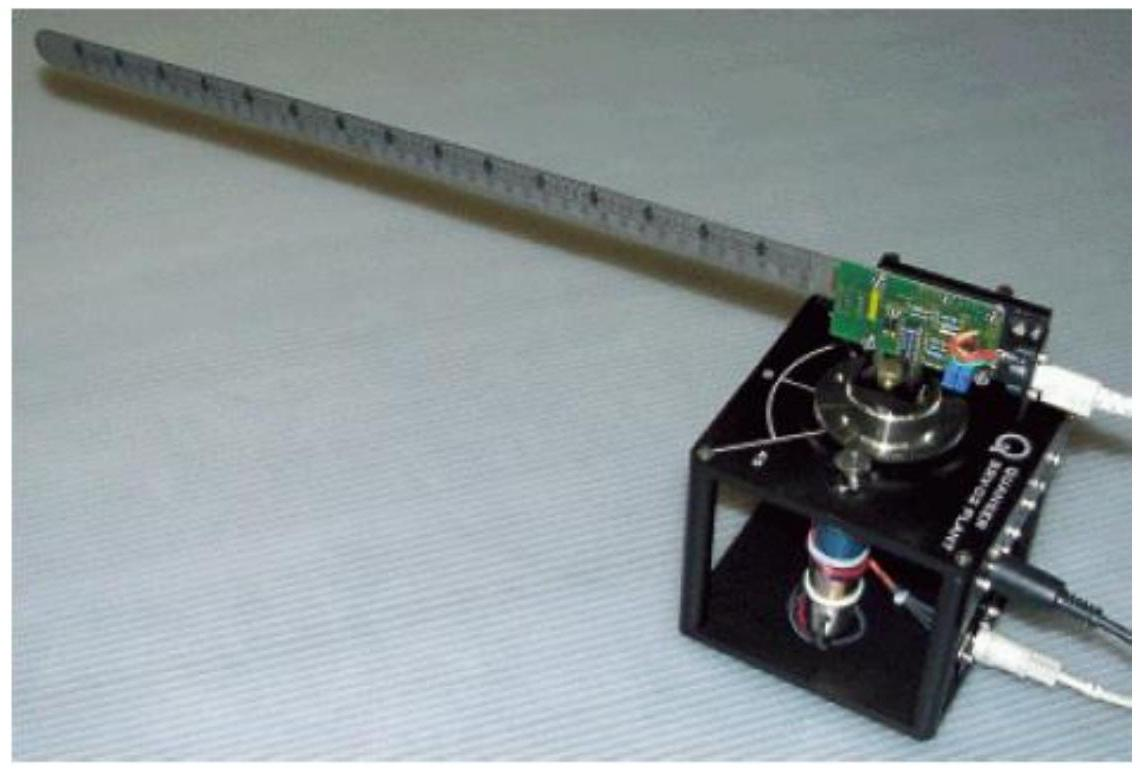
\includegraphics[width=0.45\textwidth]{Figs/2024_08_29_9e657742dc855ba919cag-01}

\vspace{15pt}
\emph{Shift CSCibLXX} %% insert here the laboratory shift you attend (L02, L03, L04 or L05)
\end{center}}

\author{ \emph{Group XX}: %% insert here the group number
    \\ \tabto{0.1cm}Name Surname | XXXXXX    %% insert here the name, surname, and IST student number of each group member
    \\ \tabto{0.1cm}Name Surname | XXXXXX
    \\ \tabto{0.1cm}Name Surname | XXXXXX
}
\date{\textbf{2026/2027 – 1st Semester}}

\begin{document}


\begin{figure}[t]
    \flushleft
    
\includegraphics[width=4cm]{Figs/ist-logo}
\end{figure}

\maketitle
\begin{center}
\textbf{Instituto Superior Técnico\\ Department of Electrical and Computer Engineering\\ Scientific Area of Systems, Decision, and Control}
\end{center}
\vspace{7pt}

\textcolor{red}{\textbf{Important notice:} This is the single report for the whole laboratory work, covering Part~I (Questions 1--3) and Part~II (Question 4). The content, counted from the Introduction to the Conclusions inclusive, may not exceed \textbf{15 pages}; anything beyond that is not evaluated. The cover, the table of contents, the declaration pages and Appendix~A do \textbf{not} count towards this limit, so use as many declaration pages as you need and do not compress the code. \textbf{Every function you create must be listed in Appendix~A.} Due at \textbf{23:59 on the day of session L12} (week~14) of your shift.}

\newpage

\section*{Declarations}
\addcontentsline{toc}{section}{{Declarations}}

\begin{tcolorbox}[declaration, title={Use of artificial intelligence}]
The laboratory work is a \textbf{green (Level~2)} component and the writing of this report is a
\textbf{yellow (Level~1)} component. Both require the declaration below. Complete it by listing
every tool used and the purpose of each use; undeclared use constitutes a breach of academic
integrity. If no AI tool was used, state so explicitly and delete the list.

\vspace{6pt}
\emph{All decisions and technical content in this work are our own. The following AI tools were
used to support the development of the work and the preparation of the report:}

\begin{itemize}
  \item \emph{[list tool] for [purpose]}          %% e.g. "for debugging the identification script"
  \item \emph{[list tool] for [purpose]}
\end{itemize}

\emph{We declare that we fully understand how all components of the work operate, including those
developed with the support of the AI tools listed above.}
\end{tcolorbox}

\vspace{10pt}

\begin{tcolorbox}[declaration, title={Originality}]
\emph{We declare that this report and the software developed are original, and that the data used
was actually obtained by the students who sign this report.}
\end{tcolorbox}

\vspace{10pt}

\begin{tcolorbox}[observation]
Each member of the group must be able to justify and explain, individually, every part of this
report. The final laboratory assessment in session~L13 consists of collective and individual
validation questions on the report, the methods used, the results obtained and the conclusions
presented. Your individual grade depends on it.
\end{tcolorbox}

\newpage
\tableofcontents
\newpage


\addcontentsline{toc}{section}{{Introduction}}
\section*{Introduction (0.5\,pts)}
\label{sec:intro}

%% Write a small introduction to the laboratory work as a whole: the plant, the control
%% objective, and how Part I and Part II fit together.


\vspace{6pt}
\noindent\rule{\textwidth}{0.8pt}\\[-4pt]
{\Large\bfseries Part I --- System Identification}\\[-6pt]
\noindent\rule{\textwidth}{0.8pt}
\addcontentsline{toc}{section}{{Part I --- System Identification}}
\vspace{4pt}

\section{Question 1 - Analyzing the problem (1.5\,pts)}
\label{sec:q1}

\subsection{Why is achieving this control objective nontrivial? (1.5\,pts)}
(\textit{Hints: Is it feasible to create a lookup table of electric voltages for the DC motor that ensures the bar tip remains at a fixed position? What would be the result if a constant voltage is applied to the motor? Would a simple feedback controller, consisting of a single gain amplifying the tracking error, effectively address the problem? Reflect on the dynamics of the motor and the bar. What might the approximate open-loop pole distribution of the system look like?})
\vspace{15pt}

%%Write your answer here


\section{Question 2 - Interfacing the plant with the computer (2.5\,pts)}
\label{sec:q2}

\subsection{Comment on the motor operation. Explain in particular why their angular position never stabilizes when its command signal is constant in the open loop conditions described. (0.5\,pts)}
\vspace{10pt}

%%Write your answer here

\subsection{Explain the procedure carried out to perform sensor calibration. (2\,pts)}
(\textit{Check the laboratory work guide to see what you should include in this answer.})
\vspace{15pt}

%%Write your answer here


\section{Question 3 - Model identification and validation (4.5\,pts)}
\label{sec:q3}

\subsection{Explanation on the tests performed on the plant to obtain the data used for identification. Discuss the results obtained with different types of excitation signals and the effect of very small amplitude and very large amplitude excitation signals. (1\,pt)}
\vspace{10pt}

%%Write your answer here

\subsection{Discussion of the sampling frequency. (0.5\,pts)}
\vspace{10pt}

%%Write your answer here

\subsection{Effect on identification of filtering the data. (0.5\,pts)}
\vspace{10pt}

%%Write your answer here

\subsection{Explanation on how the pole at the origin has been dwelt with. (0.5\,pts)}
\vspace{10pt}

%%Write your answer here

\subsection{Discussion on how the model orders have been decided. Take into consideration that the plant results from the interconnection of a DC motor and the flexible bar and discuss the models needed for each of them. (0.5\,pts)}
\vspace{10pt}

%%Write your answer here

\subsection{Description of the final ARMAX model and of the final state-space model. (0.5\,pts)}
\vspace{10pt}

%%Write your answer here

\subsection{Characterization of the plant open loop pole-zero plot, frequency response and time response of the model. (0.5\,pts)}
\vspace{10pt}

%%Write your answer here

\subsection{Model validation. (0.5\,pts)}
\vspace{10pt}

%%Write your answer here


\vspace{6pt}
\noindent\rule{\textwidth}{0.8pt}\\[-4pt]
{\Large\bfseries Part II --- Controller Design and Implementation}\\[-6pt]
\noindent\rule{\textwidth}{0.8pt}
\addcontentsline{toc}{section}{{Part II --- Controller Design and Implementation}}
\vspace{4pt}

\section{Question 4 - Controller design and testing of the controlled system (8.5\,pts)}
\label{sec:q4}

\subsection{Insert the MATLAB scripts, comments included. (0.5\,pts)}
(\textit{Place the scripts in Appendix~\ref{app:scripts} and refer to them here.})
\vspace{10pt}

%%Write your answer here

\subsection{Show and describe the block diagram used to control the system. (1\,pt)}
\vspace{10pt}

%%Write your answer here

\subsection{Comment on the choice of the weights on the quadratic cost when using the LQG design approach. Include the root-square locus. (1.5\,pts)}
\vspace{10pt}

%%Write your answer here

\subsection{Explain the effect of the choice of the noise covariance matrices in a LTR framework. (1.5\,pts)}
\vspace{10pt}

%%Write your answer here

\subsection{Display and analyze the resulting closed-loop frequency response and time response. (1.5\,pts)}
\vspace{10pt}

%%Write your answer here

\subsection{Comment on the effect of the inclusion of a pre-filter. (1\,pt)}
\vspace{10pt}

%%Write your answer here

\subsection{Discuss how do you evaluate the performance of your control system and what are the limits of performance. (1.5\,pts)}
\vspace{10pt}

%%Write your answer here


\addcontentsline{toc}{section}{{Conclusions}}
\section*{Conclusions (1\,pt)}

%% Draw some conclusions about the laboratory work as a whole. Relate what you obtained in
%% Part II back to the model you identified in Part I.


\vspace{20pt}
\begin{tcolorbox}[mybox, title={Presentation (1.5\,pts)}]
Awarded across the whole report. Every graph must display the units on both axes and carry a
caption that identifies the experimental conditions to which it refers. Answers must be direct,
concise and short, but insightful and technically correct.
\end{tcolorbox}


\newpage
\appendix
\section{MATLAB scripts}
\label{app:scripts}

This appendix does not count towards the 15-page limit, so there is no reason to shorten or
omit code. It must contain the three scripts described in the laboratory guide ---
identification, controller design, and controller testing --- \textbf{and every function you
created}, whether or not it is called by those three scripts. Use one \texttt{lstlisting}
environment per file, with the file name in the caption, and keep the comments in the code.

\begin{lstlisting}[caption={\texttt{identification.m} --- script for model identification.}]
% your code here
\end{lstlisting}

\begin{lstlisting}[caption={\texttt{controller\_design.m} --- script for controller design.}]
% your code here
\end{lstlisting}

\begin{lstlisting}[caption={\texttt{controller\_test.m} --- script for controller testing.}]
% your code here
\end{lstlisting}

\begin{lstlisting}[caption={\texttt{yourFunctionName.m} --- one listing per function you created.}]
% your code here
\end{lstlisting}


\end{document}
